\documentclass[
oneside,					% Impressão apenas no anverso. Oposto a twoside
a4paper,					% Tamanho do papel
english,					% Idioma adicional para hifenização
brazil,					% O ultimo idioma indicado será o principal idioma do documento    
]{abntex2}

\usepackage[utf8]{inputenc}
\usepackage{scalefnt}			% Permite redimensionar tamanho da fonte

\renewcommand*\familydefault{\sfdefault}
\usepackage{amsfonts, amssymb, amsmath, dsfont}		% fontes e símbolos matemáticos
\usepackage{lscape}				% Permite páginas em modo "paisagem"
\usepackage{indentfirst}		% Indenta o primeiro parágrafo de cada seção.
\usepackage{microtype} 			% Melhora a justificação do documento
\usepackage{breakurl}			% Permite quebra de linha em URLs longas
\usepackage{balance}			% Balanceia o texto no artigo
\usepackage{verbatim}			% Permite apresentar texto tal como escrito no documento, ainda que sejam comandos Latex
\usepackage{hyperref} 			% Usado para criar “hyperlinks” no PDF
\usepackage{lettrine} 			% Lettrine é a primeira letra do início de um texto que é aumentada em relação às demais
\usepackage{graphicx}			% Inclusão de gráficos e figuras
\usepackage[brazilian,hyperpageref]{backref}
\usepackage{csvsimple}
\usepackage{float}
\hypersetup{hidelinks}
\usepackage{listings}
\usepackage{float}



\titulo{Trabalho Prático}
%\title{Title in English}

\autor{Lucas de Aguilar Junqueira Campos\\Matheus Barcelos de Oliveira}
\instituicao{CENTRO FEDERAL DE EDUCAÇÃO TECNOLÓGICA DE MINAS GERAIS}
\local{Belo Horizonte}
\data{04 de dezembro de 2015}
    
\begin{document}
\frenchspacing
\pretextual
\imprimircapa 


\newpage

\pdfbookmark[0]{\contentsname}{toc}
\tableofcontents*
\newpage
\listoffigures


\newpage

\textual
\chapter{Introdução}
O presente trabalho tem como objetivo aplicar teorias de controle desenvolvidas na disciplina de Controle Digital de Sistemas Dinâmicos para analisar o determinado circuito:

\begin{figure}[H]
	\centering
	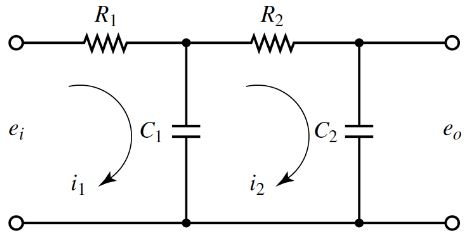
\includegraphics[\width=\textwidth]{circuito.jpg}
	\caption{Circuito objetivo}
\end{figure}

No circuito acima foram utilizados capacitores de 220 nF e resistências de 100K$\Omega$ .
Além disso são implementados três diferentes controladores, um controlador Proporcional, um controlador Proporcional Integrativo e um controlador Dahlin.

\chapter{Metodologia}
\section{Análise do Circuito}
A partir do circuito da figura 1, foram obtidos as seguintes equações diferenciais através das leis dos nós e das malhas de Kirchhoff:

\begin{equation}
	\frac{dV_{C_1}}{dt} = - \frac{R_1+R_2}{C_1 R_1^2}V_{C_1} + \frac{1}{C_1 R_1} V_{C_2} + \frac{R_2}{C_1 R_1^2} e_i
\end{equation}
\begin{equation}
	\frac{dV_{C_2}}{dt} = \frac{1}{C_2 R_2} V_{C_1} - \frac{1}{C_2 R_2}V_{C_2}
\end{equation}
\begin{equation}
	e_o = V_{C_2}
\end{equation}

A partir das equações foi obtido a seguinte representação em espaço de estados:

\begin{equation}
	\left[
	\begin{matrix}
	\dot{V_{C_1}}\\\dot{V_{C_2}}
	\end{matrix}
	\right]
	= 
	\left[
	\begin{matrix}
		-\frac{R_1+R_2}{C_1 R_1^2} & \frac{1}{C_1 R_1}\\
		\frac{1}{C_2 R_2} & -\frac{1}{C_2 R_2}
	\end{matrix}
	\right]
	\left[
	\begin{matrix}
	V_{C_1}\\V_{C_2}
	\end{matrix}
	\right]
	+ \left[
	\begin{matrix}
	\frac{R_2}{C_1 R_1^2}\\
	0
	\end{matrix}
	\right] e_i
\end{equation}	
	
\begin{equation}	
	e_o = \left[
	\begin{matrix}
		0 & 1
	\end{matrix}
	\right]
	\left[
	\begin{matrix}
		V_{C_1}\\V_{C_2}
	\end{matrix}
	\right]
	+
	\left[ 0 \right]e_i
\end{equation}

\section{Função de Transferência}

A partir da representação em espaço de estados, utilizando o MATLAB, chegou-se a seguinte equação:

\begin{equation}
	G(s) = \frac{2066}{s^2 + 136,4s + 2066}
\end{equation}

\section{Projeto de Controlador por Alocação de Polos}

A função de transferência da malha fechada foi obtida utilizando a seguinte definição:

\begin{equation}	
T(s) = \frac{D(s)G(s)}{1 + D(s)G(s)}
\end{equation}

Sendo:
T(s): função de transferência da malha fechada;
G(s): função de transferência da malha aberta;
D(s): função do controlador.

Assim, definindo 
\begin{equation} 
D(s) = K_p
\end{equation}
obteve-se a seguinte função de transferência da malha fechada:

\begin{equation} 
T(s) = \frac{2066K_p}{s^2 + 136,4s + (K_p +1)2066}
\end{equation}

A partir da equação temos que:

\begin{equation}
\zeta = \frac{68.2}{w_s}
\end{equation}

Para que o sistema se torne oscilatório, $K_p$ deve respeitar a seguinte inequação:

\begin{equation}
0 < \frac{68.2}{w_s} < 1
\end{equation} 

Isso implica que:

\begin{equation}
K > 1.2513
\end{equation}

Para se escolher uma constante de tempo para a discretização deve-se escolher uma constante menor que:

\begin{equation}
T < 2/w_s
\end{equation}

\begin{equation}
T < 0.0147 s
\end{equation}


\section{Função de Transferência da Malha Fechada}


Utilizando $K_p$ como 10, chegamos à equação:

\begin{equation}
	T(s) =  \frac{20660}{s^2 + 136.4 s + 22726}
\end{equation}


Discretizando a função de transferência contínua anterior e constante de tempo T = 0.0018 s, a T(z) foi definida como:

\begin{equation} 
T(z) = \frac{0.0307 z + 0.02829}{z^2 - 1.717 z + 0.7823}
\end{equation}

Para projetar os controladores a seguir será utilizada como planta as funções de transferência acima.

\section{Projeto controlador PI}

O controlador Proporcional e Integral (PI) foi modelado seguindo as definições a seguir:

\begin{equation} 
D(z) = K_p + K_i \frac{1}{z-1}
\end{equation}
\begin{equation} 
K_i = \frac{K_p T}{T_i}
\end{equation}

Em que:
Kp: constante da ação proporcional;
Ki: constante da ação integral;
T: 	tempo de amostragem;
Ti:	tempo de integração.


Com o objetivo de eliminar as oscilações do sistema, eliminar o erro em estado estacionário e possibilitar que o sistema responda mais rapidamente foram definidos os valores de $K_p$ e $K_i$, que foram:

\begin{equation} 
K_p = 0,023404
\end{equation}
\begin{equation} 
T_i = 0,0009
\end{equation}

O que leva a seguinte ação de controle:

\begin{equation}
	D_{PI}(z) = 0.023404 + 0.0468 \frac{1}{z-1} 
\end{equation}

Assim, a função de transferência da malha fechada obtida foi:

\begin{equation} 
T_{PI}(z) = \frac{0,0007186(z+1)(z+0,9213)}{(z-0,9509)(z^2 - 1,766z + 0,822)}
\end{equation}

\section{Projeto controlador Dahlin}

O controlador de Dahlin foi modelado seguindo as seguintes definições:

\begin{equation} 
\tau = 0,01
\end{equation}
\begin{equation} 
k = 1
\end{equation}
\begin{equation} 
q = e^{-\frac{T}{\tau}}
\end{equation}
\begin{equation} 
D_{Dahlin}(z) = \frac{1}{G(z)}\frac{(1-q)z^{-k}}{1-qz^{-1}-(1-q)z^{-k}}
\end{equation}

Assim, após a realização dos cálculos, com $\tau$ igual a 0,01 s e k=1 devido ao atraso intrínseco, a função do controlador Dahlin foi definida como:

\begin{equation} 
D_{Dahlin}(z) = \frac{5,365 (z^2 - 1,717z + 0,7823)}{ (z+0.9213) (z-1)}
\end{equation}

Fechando a malha, obteve-se a seguinte função de transferência pulsada para malha fechada:

\begin{equation} 
T_{Dahlin}(z) = \frac{0,16473}{z-0.8353}
\end{equation}


\chapter{Resultados}

\section{Resposta do sistema à uma entrada em degrau}

Simulando o sistema discretizado, obteve-se o seguinte resultado:

\begin{figure}[H]
	\centering
	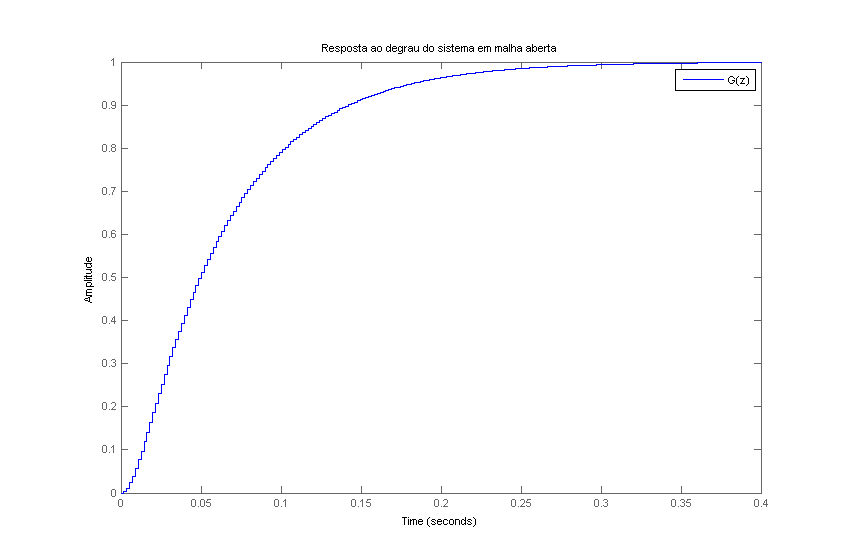
\includegraphics[scale = 0.7]{malhaAbertaSimulacao.png}
	\caption{Resultado da simulação do sistema em malha aberta}
\end{figure}

Após a medição com auxílio do osciloscópio foi criado o seguinte gráfico comparativo:

 \begin{figure}[H]
 	\centering
 	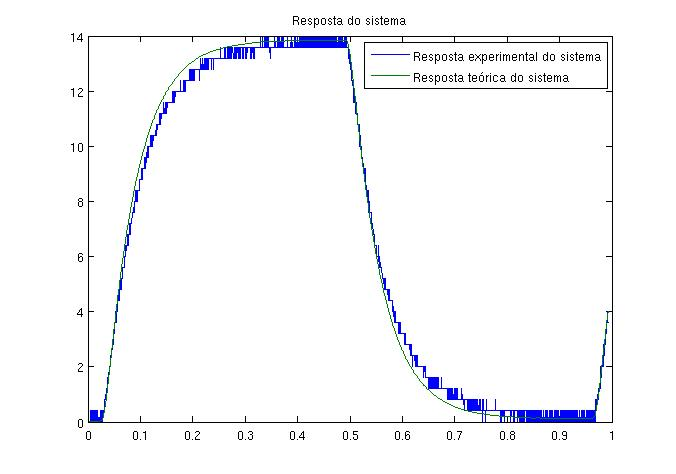
\includegraphics[scale = 0.7]{Respostas.jpg}
 	\caption{Comparação resultado experimental e teórico}
 \end{figure}

\section{Resposta pulsada do sistema ao controlador por alocação de polos}

Comparando o resultado da simulação com o experimental, observa-se a seguinte similiaridade entre as duas respostas:

\begin{figure}[H]
	\centering
	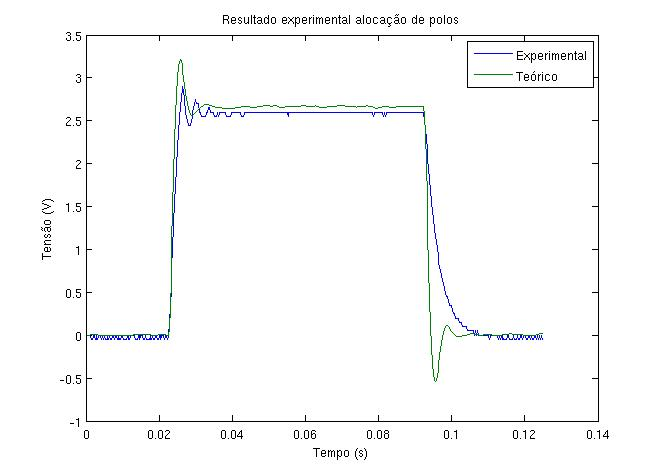
\includegraphics[scale = 0.7]{Resposta_Proporcional.jpg}
	\caption{Comparação resultado experimental e teórico para controlador por alocação de polos digital}
\end{figure}

\section{Controlador PI}

Após a modelagem do controlador PI, simulou-se o sistema afim de verificar a modelagem desenvolvida e comparar o resultado com a simulação do sistema com o controlador por alocação de polos. Com o auxílio do MATLAB, a simulação obteve o seguinte resultado: 

\begin{figure}[H]
	\centering
	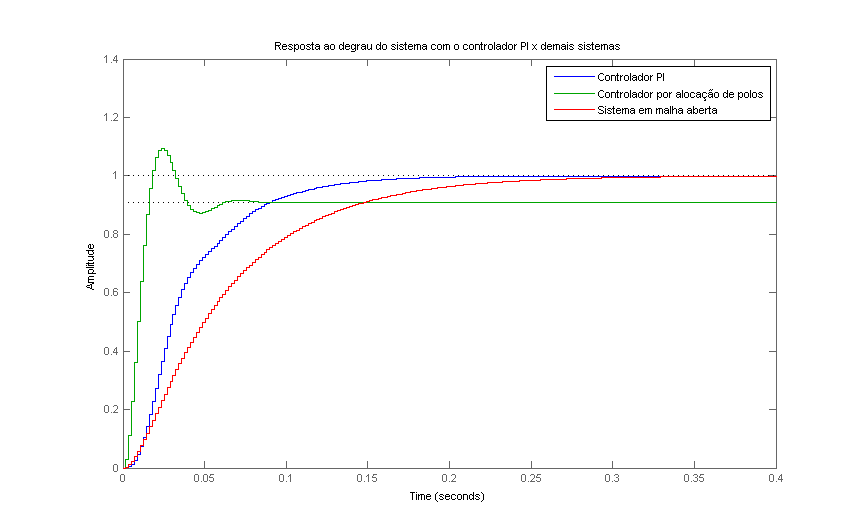
\includegraphics[scale = 0.7]{controladorPISimulacao.png}
	\caption{Resultado da simulação do controlador PI x demais sistemas}
\end{figure}

\begin{figure}[H]
	\centering
	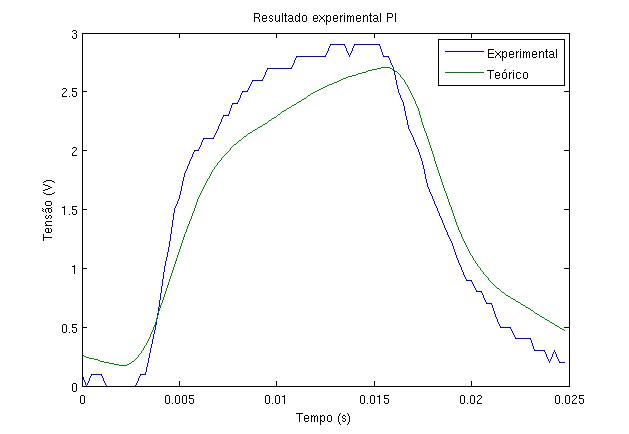
\includegraphics[scale = 0.7]{Resposta_PI.jpg}
	\caption{Comparação entre resultado teórico e experimental para o controlador PI}
\end{figure}

Analisando o gráfico, pode-se constatar que o sistema utilizando o controlador PI eliminou o erro em estado estacionário, em relação ao controlador por alocação de polos, e obteve resposta mais rápida em relação ao sistema em malha aberta, utilizando os devidos valores de Kp e Ki calculados.

\section{Controlador Dahlin}

Comparou-se as respostas do sistema com um controlador de ganho proporcional igual a 10, com um controlador de Dahlin e a resposta do sistema em malha aberta, resultando no seguinte gráfico comparativo:

\begin{figure}[H]
	\centering
	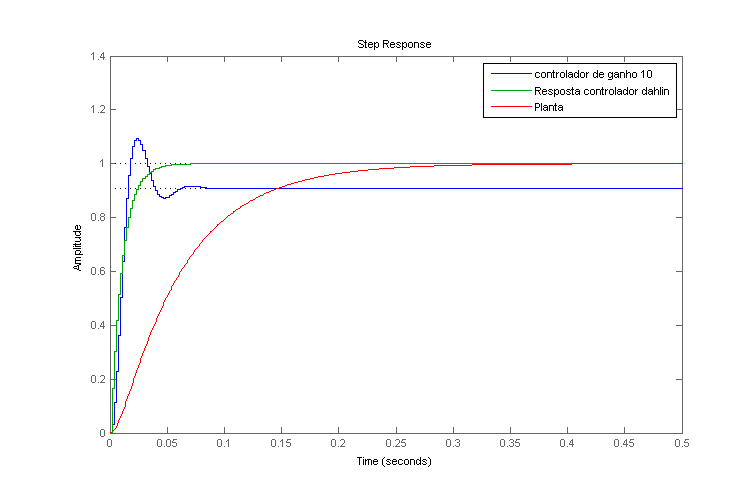
\includegraphics[scale = 0.7]{dahlinSimulacao.png}
	\caption{Resultado da simulação do sistema utilizando o controlador de Dahlin}
\end{figure}

Observa-se que o controlador de Dahlin respondeu mais rapidamente que os outros, eliminando o erro de estado estacionário do controlador proporcional.

\postextual
\begin{apendicesenv}
	\chapter{Controlador Proporcional}
	\lstinputlisting[language=C]{Controlador_Proporcional_RC.ino}
	\chapter{Controlador Proporcional Integrativo}
	\lstinputlisting[language=C]{Controlador_PI.ino}
	\chapter{Controlador Dahlin}
	\lstinputlisting[language=C]{Dahlin.ino}	
\end{apendicesenv}


\end{document}          
